\chapter{Disain}
\label{chap:disain}

\section{Disain Antarmuka}
\label{sec:disainantarmuka}

\hspace{0,5cm}Pada sub-bab ini akan dibahas mengenai disain antar muka aplikasi \textit{mobile} dan \textit{website}.

\subsection{Disain Aplikasi \textit{Mobile}}
\label{subsec:disainaplikasimobile}

\hspace{0,5cm}Pada aplikasi \textit{mobile} terdapat beberapa halaman utama pendukung fitur, yakni:
\begin{enumerate}
	\item Halaman \textit{login}
	\item	Halaman pendaftaran
	\item Halaman pengisian profil rumah tangga
	\item Halaman \textit{dashboard}
	\item Halaman penambahan anggota
	\item Halaman anggota keluarga
	\item Halaman pengolahan kategori transaksi
	\item Halaman penambahan kategori
	\item Halaman transfer
	\item Halaman penambahan pemasukan
	\item Halaman penambahan pengeluaran
	\item Halaman pemilihan laporan
	\item Halaman laporan
\end{enumerate}

\begin{figure}
\centering
\resizebox{\textwidth}{!}{
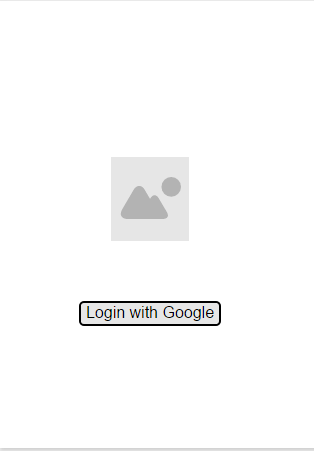
\includegraphics[scale=0.01]{Gambar/mockup/login}
}
\caption[Tampilan \textit{login}]{Tampilan \textit{login}} 
\label{fig:design_app_login}
\end{figure}

\begin{figure}
\centering
\resizebox{\textwidth}{!}{
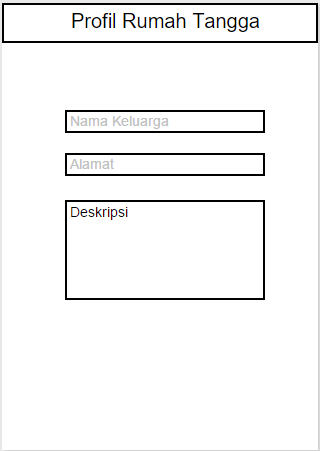
\includegraphics[scale=0.01]{Gambar/mockup/data_rumah_tangga}
}
\caption[Tampilan pengisian profil rumah tangga]{Tampilan pengisian profil rumah tangga} 
\label{fig:design_app_profil awal}
\end{figure}

\begin{figure}
\centering
\resizebox{\textwidth}{!}{
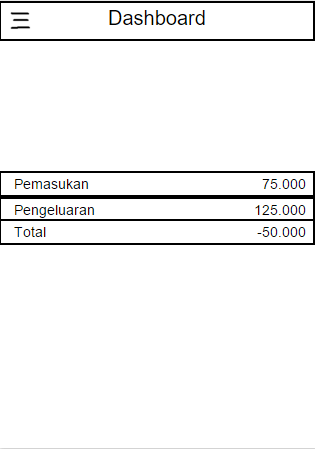
\includegraphics[scale=0.01]{Gambar/mockup/dashboard}
}
\caption[Tampilan \textit{dashboard}]{Tampilan \textit{dashboard}} 
\label{fig:design_app_dashboard}
\end{figure}

\begin{figure}
\centering
\resizebox{\textwidth}{!}{
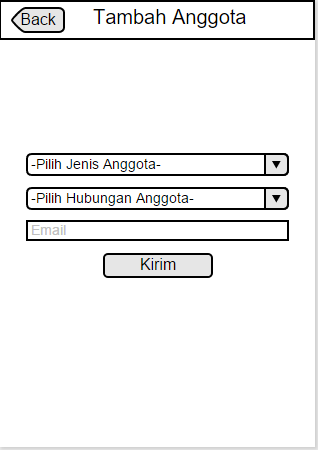
\includegraphics[scale=0.01]{Gambar/mockup/tambah_anggota}
}
\caption[Tampilan penambahan anggota]{Tampilan penambahan anggota} 
\label{fig:design_app_penambahan_anggota}
\end{figure}

\begin{figure}
\centering
\resizebox{\textwidth}{!}{
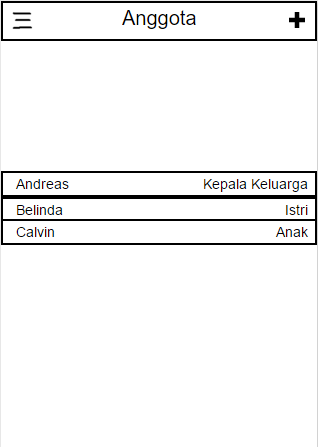
\includegraphics[scale=0.01]{Gambar/mockup/anggota}
}
\caption[Tampilan anggota keluarga]{Tampilan anggota keluarga} 
\label{fig:design_app_anggota_keluarga}
\end{figure}

\begin{figure}
\centering
\resizebox{\textwidth}{!}{
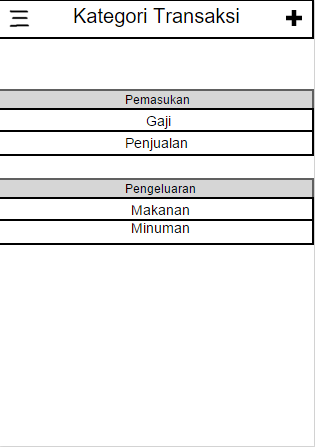
\includegraphics[scale=0.01]{Gambar/mockup/kategori_transaksi}
}
\caption[Tampilan pengolahan kategori transaksi]{Tampilan pengolahan kategori transaksi} 
\label{fig:design_app_kategori_transaksi}
\end{figure}

\begin{figure}
\centering
\resizebox{\textwidth}{!}{
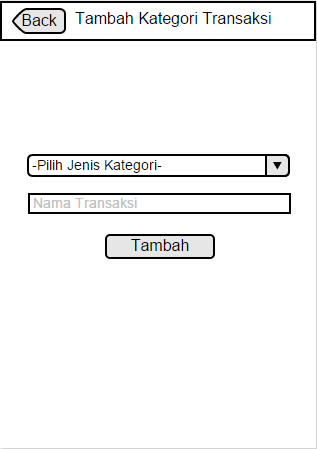
\includegraphics[scale=0.01]{Gambar/mockup/tambah_kategori_transaksi}
}
\caption[Tampilan penambahan kategori]{Tampilan penambahan kategori} 
\label{fig:design_app_penambahan_kategori}
\end{figure}

\begin{figure}
\centering
\resizebox{\textwidth}{!}{
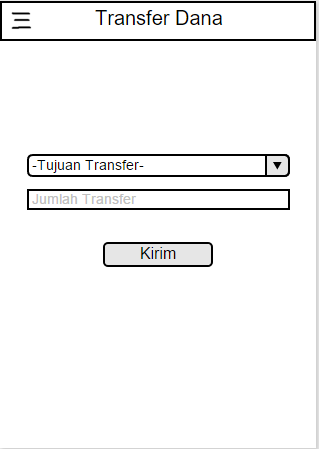
\includegraphics[scale=0.01]{Gambar/mockup/transfer_dana}
}
\caption[Tampilan transfer]{Tampilan transfer} 
\label{fig:design_app_transfer}
\end{figure}

\begin{figure}
\centering
\resizebox{\textwidth}{!}{
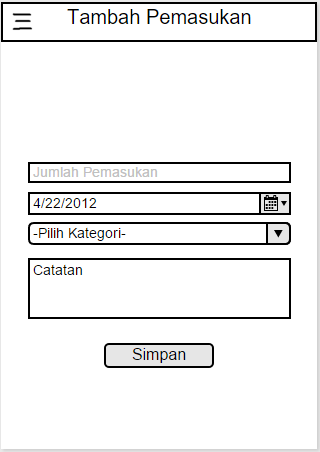
\includegraphics[scale=0.01]{Gambar/mockup/tambah_pemasukan}
}
\caption[Tampilan penambahan pemasukan]{Tampilan penambahan pemasukan} 
\label{fig:design_app_penambahan_pemasukan}
\end{figure}

\begin{figure}
\centering
\resizebox{\textwidth}{!}{
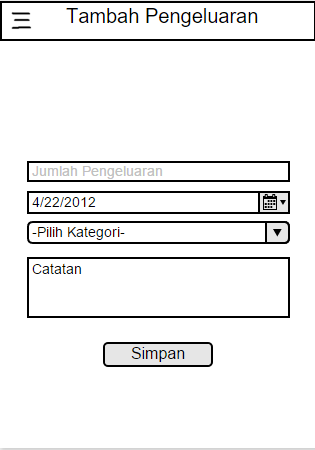
\includegraphics[scale=0.01]{Gambar/mockup/tambah_pengeluaran}
}
\caption[Tampilan penambahan pengeluaran]{Tampilan penambahan pengeluaran} 
\label{fig:design_app_penambahan_pengeluaran}
\end{figure}

\begin{figure}
\centering
\resizebox{\textwidth}{!}{
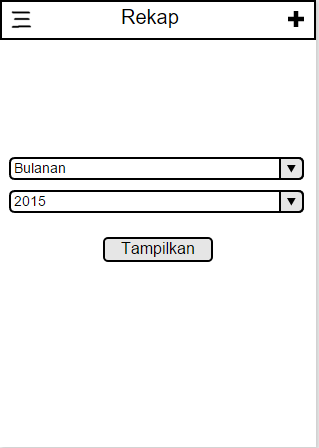
\includegraphics[scale=0.01]{Gambar/mockup/rekap}
}
\caption[Tampilan pemilihan laporan]{Tampilan pemilihan laporan} 
\label{fig:design_app_pemilihan_laporan}
\end{figure}

\begin{figure}
\centering
\resizebox{\textwidth}{!}{
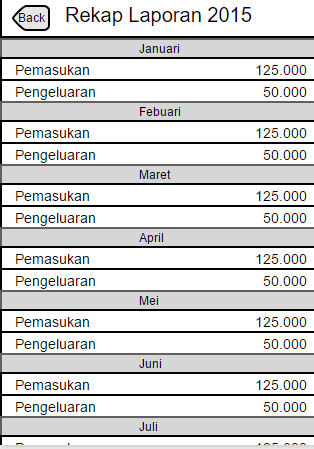
\includegraphics[scale=0.01]{Gambar/mockup/rekap_laporan}
}
\caption[Tampilan laporan]{Tampilan laporan} 
\label{fig:design_app_laporan}
\end{figure}

\subsection{Disain Apliasi \textit{Website}}
\label{subsec:disainaplikasiwebsite}

\hspace{0,5cm}Pada aplikasi \textit{website} terdapat beberapa halaman utama pendukung fitur, yakni;
\begin{enumerate}
	\item Halaman \textit{login}
	\item Halaman \textit{dashboard}
	\item Halaman daftar rumah tangga
	\item Halaman pengololahan kategori transaksi
	\item Halaman pelaporan
\end{enumerate}

\begin{figure}
\centering
\resizebox{\textwidth}{!}{
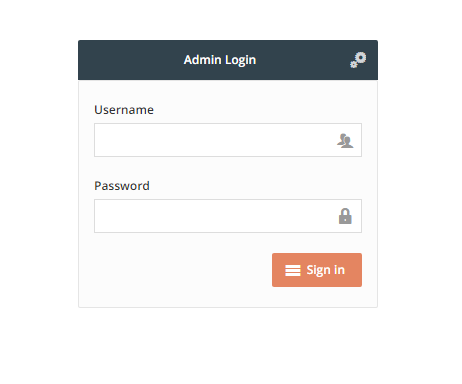
\includegraphics[scale=0.01]{Gambar/design-web/login}
}
\caption[Tampilan login]{Tampilan login} 
\label{fig:design_web_login}
\end{figure}

\begin{figure}
\centering
\resizebox{\textwidth}{!}{
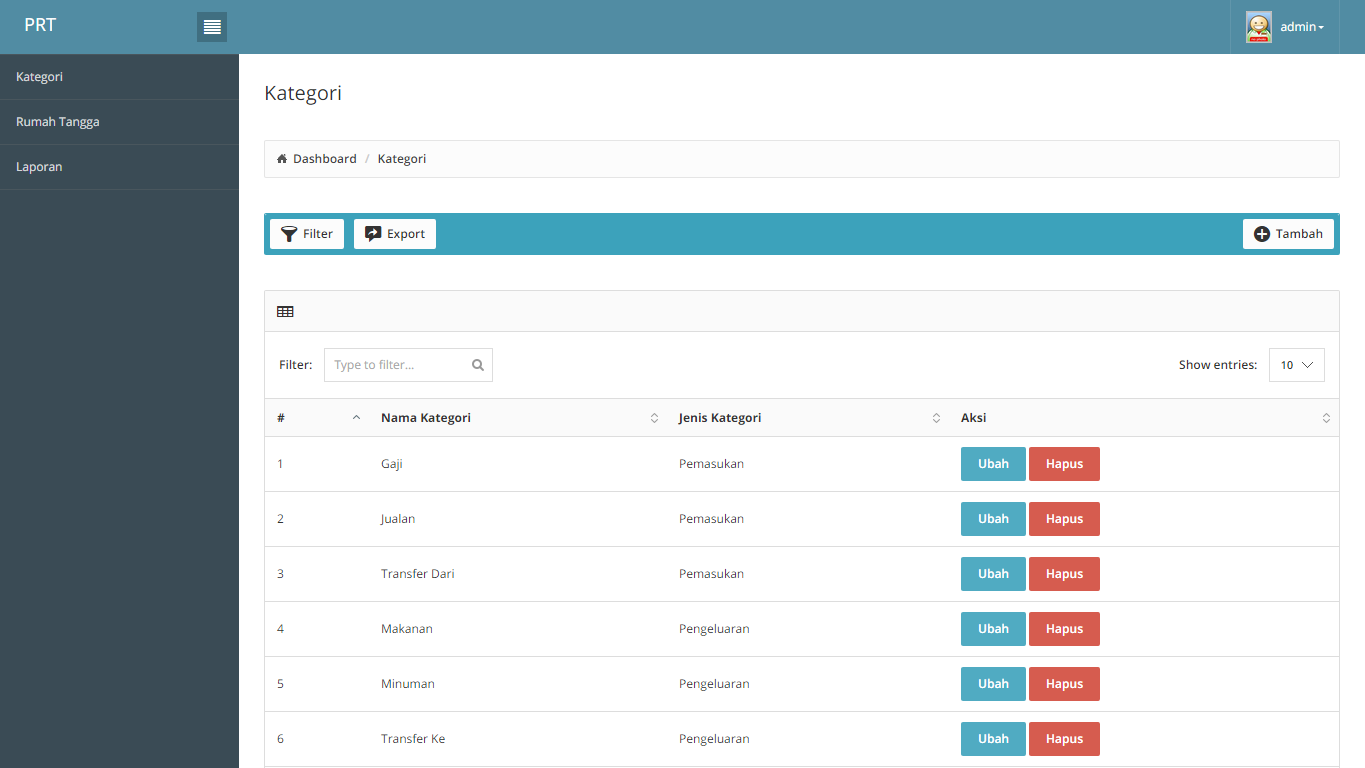
\includegraphics[scale=0.01]{Gambar/design-web/index_kategori}
}
\caption[Tampilan halaman kategori]{Tampilan halaman kategori} 
\label{fig:design_web_index_kategori}
\end{figure}

\begin{figure}
\centering
\resizebox{\textwidth}{!}{
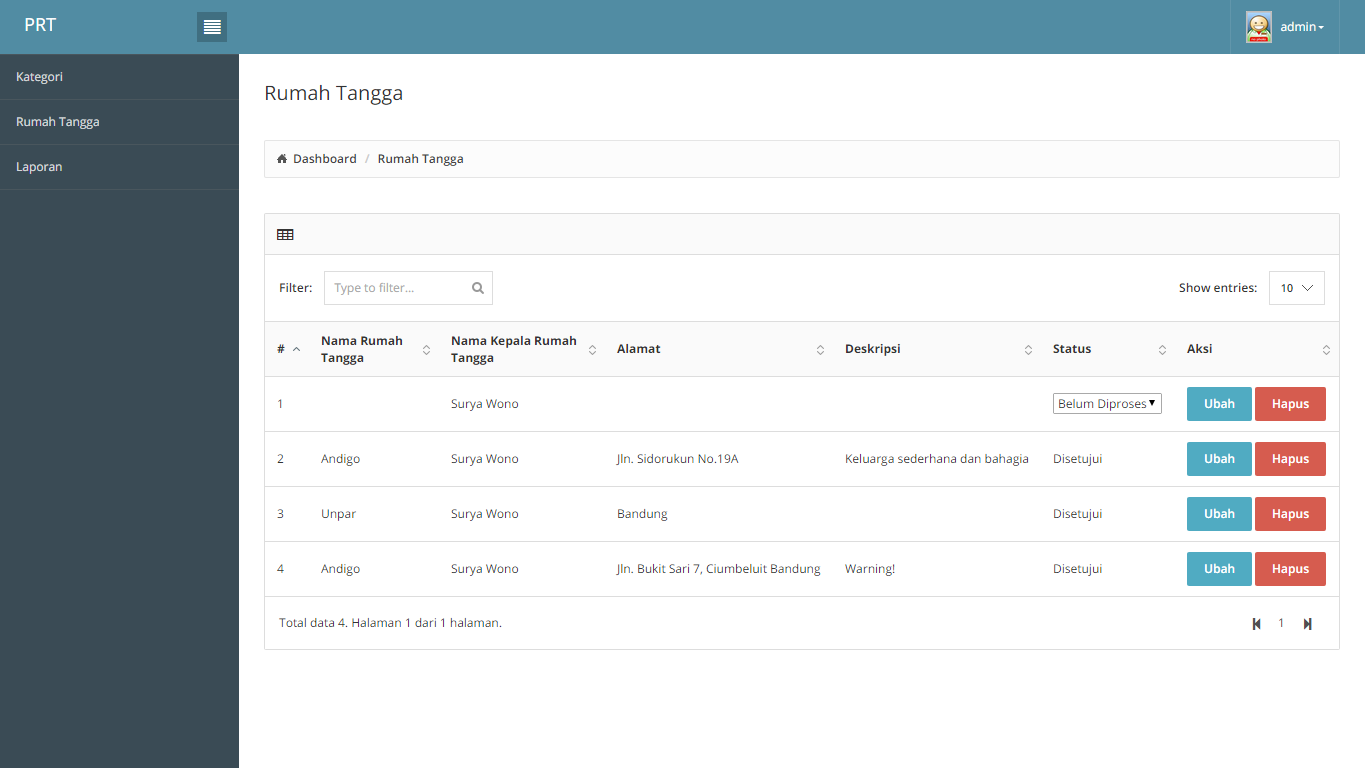
\includegraphics[scale=0.01]{Gambar/design-web/index_rumah_tangga}
}
\caption[Tampilan halaman rumah tangga]{Tampilan halaman rumah tangga} 
\label{fig:design_web_index_rumah_tangga}
\end{figure}

\section{Disain \textit{Webservice}}

\hspace{0,5cm}Pada webservice ini, terdapat dua peristiwa utama yaitu \textit{request} dan \textit{response}.Request akan memiliki beberapa parameter sesuai fungsi yang digunakan. Response yang dikembalikan dari \textit{webservice} berupan JSON dan memiliki format sesuai dengan Gambar~\ref{fig:format_response_webservice} dimana terdapat atribut utama yaitu \textit{response} yang membungkus tiga atribut lainnya yaitu status yang merupakan kode status dari \textit{request}, message yang merupakan keterangan status dan data yang merupakan atribut yang membungkus nilai-nilai yang dikembalikan.

\begin{lstlisting} [caption= Format \textit{response}  webservice]
{
	"response":{
		"status": (kode status),
		"message": (keterangan status),
		"data": {
			...
		}
	}
}
\end{lstlisting}

\textit{Request} dan \textit{response} pada \textit{webservice} untuk setiap fungsi akan dijelaskan sebagai berikut:
\begin{enumerate}
	\item Login (POST)
		\begin{itemize}
			\item Request pada Tabel~\ref{tab:request_login}
				\begin{table}[h]
					\centering
						\begin{tabular}{ |p{4cm}|p{10cm}|}
							\hline
							parameter & nilai \\ \hline
							email & email yang digunakan saat mendaftar \\ \hline
							password & password yang didaftarkan \\ \hline
					\end{tabular}
					\caption{\textit{Request login}}
					\label{tab:request_login}
				\end{table}
			\item Response pada Tabel~\ref{tab:response_login}
				\begin{table}[h]
					\centering
						\begin{tabular}{ |p{4cm}|p{10cm}|}
							\hline
							atribut & nilai \\ \hline
							status & 202 / 402 \\ \hline
							message & Login berhasil / Login gagal \\ \hline
							data & [data anggota dan rumah tangga] \\ \hline
						\end{tabular}
						\caption{\textit{Response login}}
					\label{tab:response_login}
				\end{table}
		\end{itemize}
		
		\item Menambah transaksi (POST)
		\begin{itemize}
			\item Request pada Tabel~\ref{tab:request_tambah_transaksi}
				\begin{table}[h]
					\centering
						\begin{tabular}{ |p{4cm}|p{10cm}|}
							\hline
							parameter & nilai \\ \hline
							kategori\_id & id kategori yang dipilih \\ \hline
							besaran & nilai transaksi \\ \hline
							deskripsi & deskripsi transaksi \\ \hline
							waktu & waktu transaksi \\ \hline
							anggota\_id & id anggota \\ \hline
					\end{tabular}
					\caption{\textit{Request} penambahan transaksi}
					\label{tab:request_tambah_transaksi}
				\end{table}
			\item Response pada Tabel~\ref{tab:response_tambah_transaksi}
				\begin{table}[h]
					\centering
						\begin{tabular}{ |p{4cm}|p{10cm}|}
							\hline
							atribut & nilai \\ \hline
							status & 200\\ \hline
							message & Berhasil disimpan \\ \hline
							data & [data sesuai request] \\ \hline
						\end{tabular}
						\caption{\textit{Request} penambahan transaksi}
					\label{tab:response_tambah_transaksi}
				\end{table}
		\end{itemize}
		
		\item Menyiapkan data laporan (GET)
		\begin{itemize}
			\item Request pada Tabel~\ref{tab:request_laporan}
				\begin{table}[h]
					\centering
						\begin{tabular}{ |p{4cm}|p{10cm}|}
							\hline
							parameter & nilai \\ \hline
							jenis & jenis laporan (tahun \& bulan) \\ \hline
							anggota\_id & id anggota \\ \hline
							tahun (untuk jenis bulanan) & tahun laporan \\ \hline
							bulan (untuk jenis mingguan) & minggu laporan \\ \hline
					\end{tabular}
					\caption{\textit{Request} penyiapan data laporan}
					\label{tab:request_laporan}
				\end{table}
			\item Response pada Tabel~\ref{tab:response_laporan}
				\begin{table}[h]
					\centering
						\begin{tabular}{ |p{4cm}|p{10cm}|}
							\hline
							atribut & nilai \\ \hline
							status & 400\\ \hline
							message & Data found \\ \hline
							data & [data laporan] \\ \hline
						\end{tabular}
						\caption{\textit{Response} penyiapan data laporan}
					\label{tab:response_laporan}
				\end{table}
		\end{itemize}
\end{enumerate}

\section{Disain Basis Data}
\label{sec:disainbasisdata}

\hspace{0,5cm}Pada sub-bab ini akan digambarkan disain basis data berupa \textit{Entity Relational Diagram} untuk aplikasi pembukuan rumah tangga dan \textit{website} pengolahan aplikasi pada Gambar~\ref{fig:er_diagram_prt}.

\begin{figure}[h]
\centering
\resizebox{\textwidth}{!}{
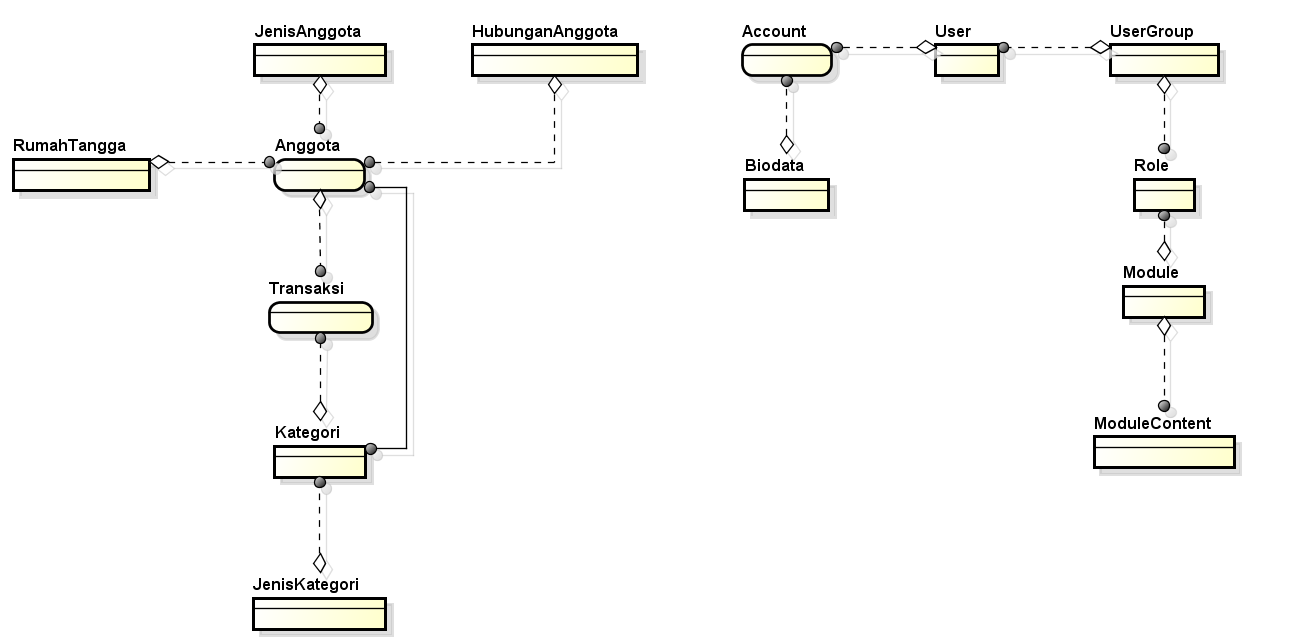
\includegraphics[scale=0.01]{Gambar/er-diagram}
}
\caption[\textit{Entity Relational Diagram} Pembukuan Rumah Tangga]{\textit{Entity Relational Diagram} Pembukuan Rumah Tangga} 
\label{fig:er_diagram_prt}
\end{figure}


